%% LaTeX Beamer presentation template (requires beamer package)
%% see http://bitbucket.org/rivanvx/beamer/wiki/Home
%% idea contributed by H. Turgut Uyar
%% template based on a template by Till Tantau
%% this template is still evolving - it might differ in future releases!

\documentclass[aspectratio=169]{beamer}
\usefonttheme[onlymath]{serif}
\mode<presentation>
{
\usetheme{Warsaw}

\setbeamercovered{transparent}
\usecolortheme{seahorse}
}

\usepackage[english]{babel}
\usepackage[latin1]{inputenc}

% font definitions, try \usepackage{ae} instead of the following
% three lines if you don't like this look
\usepackage{mathptmx}
\usepackage[scaled=.90]{helvet}
\usepackage{courier}
\usepackage{color}
\usepackage{ragged2e}

\usepackage[T1]{fontenc}


\title[IEEE AP-S/URSI 2016]{An Approximate Exponentiated Weibull Joint Envelope-Phase Distribution}

%\subtitle{}

% - Use the \inst{?} command only if the authors have different
%   affiliation.
%\author{F.~Author\inst{1} \and S.~Another\inst{2}}
\author[An Approximate Exponentiated Weibull Joint Envelope-Phase Distribution]{\textbf{Jos\'e V. M. Cardoso}, Wamberto J. L. Queiroz, and Marcelo S. Alencar}

% - Use the \inst command only if there are several affiliations.
% - Keep it simple, no one is interested in your street address.
\institute[Universities of]
{
%
Institute for Advanced Studies in Communications -- Iecom\\
Department of Electrical Engineering\\
Federal University of Campina Grande -- UFCG
}

\date{IEEE AP-S/URSI 2016 \\ Fajardo, Puerto Rico}

\defbeamertemplate*{footline}{shadow theme}
{%
  \leavevmode%
  \hbox{\begin{beamercolorbox}[wd=.5\paperwidth,ht=2.5ex,dp=1.125ex,leftskip=.3cm plus1fil,rightskip=.3cm]{author in head/foot}%
    \usebeamerfont{author in head/foot}\insertframenumber\,/\,\inserttotalframenumber\hfill\insertshortauthor
  \end{beamercolorbox}%
  \begin{beamercolorbox}[wd=.5\paperwidth,ht=2.5ex,dp=1.125ex,leftskip=.3cm,rightskip=.3cm plus1fil]{title in head/foot}%
    \usebeamerfont{title in head/foot}\insertshorttitle%
  \end{beamercolorbox}}%
  \vskip0pt%
}

% This is only inserted into the PDF information catalog. Can be left
% out.
\subject{Talks}



% If you have a file called "university-logo-filename.xxx", where xxx
% is a graphic format that can be processed by latex or pdflatex,
% resp., then you can add a logo as follows:

% \pgfdeclareimage[height=0.5cm]{university-logo}{university-logo-filename}
% \logo{\pgfuseimage{university-logo}}



% Delete this, if you do not want the table of contents to pop up at
% the beginning of each subsection:
%\AtBeginSubsection[]
%{
%\begin{frame}<beamer>
%\frametitle{Outline}
%\tableofcontents[currentsection]
%\end{frame}
%}

% If you wish to uncover everything in a step-wise fashion, uncomment
% the following command:

%\beamerdefaultoverlayspecification{<+->}

\begin{document}

\begin{frame}
\titlepage
\end{frame}

\begin{frame}
\frametitle{Outline}
\tableofcontents
% You might wish to add the option [pausesections]
\end{frame}


\section{Introduction}
\begin{frame}{Introduction}
    \begin{itemize}
        \item Free-space optical (FSO) systems
            \begin{itemize}
                \item Short range, outdoor and indoor wireless
                \item Large bandwidth, high average capacity
            \end{itemize}
        \item Major challenge: atmospheric turbulence
            \begin{itemize}
                \item Scintillation
                \item Beam Wander
                \item Beam Spreading
            \end{itemize}
        \item Improvement in performance
            \begin{itemize}
                \item Enlarge the aperture in the receiver
            \end{itemize}
        \item Statistical characterization of the laser beam
            \begin{itemize}
                \item Log-normal, Gamma-Gamma
                \item Exponentiated Weibull
            \end{itemize}
    \end{itemize}
\end{frame}

\subsection{Atmospheric Turbulence Channel Statistics}
\begin{frame}{Exponentiated Weibull Statistics}
    \begin{itemize}
        \item Barrios proposed the following model for the irradiance at the receiver:
            \begin{equation*}
                I^p \triangleq \sum_{n=1}^{m}w_nI_n^p
            \end{equation*}
            which was then approximated as
            \begin{equation*}
                I \approx \lim_{p\to \infty}\left(\sum_{n=1}^{m}w_nI_n^p\right)^{1/p} = \max \left\{I_1, I_2, ..., I_m\right\}
            \end{equation*}
        \item $I_n \thicksim$ Weibull ($\alpha$) iid $\Rightarrow I \thicksim$ Exp. Weibull($\alpha, m$)
        \item Suitable to fit weak, moderate, and strong atmospheric turbulence
        \item However, no phase information was taken into account
    \end{itemize}
\end{frame}

\begin{frame}{Phase Distribution}
    \begin{itemize}
        \item To asses the coherent detection of optical signals subject to atmospheric turbulence
        \item To compute bit error rate for communications systems using phase modulation schemes
        \item To determine optimum receiver aperture diameter
        \item Belmonte assumed Gaussian random phase fluctuations\footnote{A. Belmonte and J. M. Kahn, "Performance of synchronous optical receivers using atmospheric compensation techniques", Opt. Express, vol. 16, no. 18, pp. 14 151-14 162, Sep. 2008}
        \item Perlot assumed Beta distributed phase and also that phase and amplitude were independent\footnote{N. Perlot, "Turbulence-induced fading probability in coherent optical communication through the atmosphere," Appl. Opt. 46, 7218-7226 (2007)}
     \end{itemize}
\end{frame}


\section{Joint Envelope-Phase Probability Density Function}
\begin{frame}{Joint Envelope-Phase Density Function}
    \textit{Proposition}: Let $R \in \mathbb{R}^{+}$ and $\Theta \in \left[0,\frac{4\pi}{\alpha}\right)$, $\alpha > 0$, be random variables (rvs) representing, respectively, the envelope and the phase of the exponentiated Weibull signal with shape parameters $\alpha > 0$ and $\mu > 0$, and scale parameter $\Omega > 0$. Hence, the joint probability density function (pdf) of the random vector $(R,\Theta)$, denoted as $p_{R,\Theta}(r,\theta)$, is given by
\begin{align*}
    p_{R,\Theta}(r,\theta) = &\dfrac{(\alpha\mu)^2}{4\pi\Omega}\left(\dfrac{r}{\Omega}\right)^{\alpha-1}\exp\left(-\left(\dfrac{r}{\Omega}\right)^{\alpha}\right)\times\\
    &\left[\mathrm{erf}\left(\left(\dfrac{r}{\Omega}\right)^{\alpha/2}\Bigg|\cos\left(\dfrac{\alpha\theta}{2}\right)\Bigg|\right)\times\mathrm{erf}\left(\left(\dfrac{r}{\Omega}\right)^{\alpha/2}\Bigg|\sin\left(\dfrac{\alpha\theta}{2}\right)\Bigg|\right)\right]^{\mu-1}.
\label{eq:joint_pdf}
\end{align*}
\end{frame}

\begin{frame}{Joint Envelope-Phase Density Function}
    \textit{Proof:}
    \begin{itemize}
        \item $R \in \mathbb{R}^{+}$, $\Theta \in \left[0, \frac{4\pi}{\alpha}\right)$, $\alpha \in \mathbb{R}^{+}$
        \item $Z = X + jY \triangleq R^{\alpha/2}\exp\left(j\frac{\alpha\Theta}{2}\right)$
        \item $X = R^{\alpha/2}\cos\left(\frac{\alpha\Theta}{2}\right); ~~ Y = R^{\alpha/2}\sin\left(\frac{\alpha\Theta}{2}\right)$
        \item $X^2 \triangleq \max\limits_{1 \leq i \leq m} X_i^2 ~~\text{and} ~~ Y^2 \triangleq \max\limits_{1 \leq i \leq m} Y^2_i,~m \in \mathbb{N}$,
    \end{itemize}
    in which $X_i$ and $Y_i$ are assumed to be independent Gaussian distributed rvs with zero mean and variance $\frac{\Omega^\alpha}{2}$, representing the scattered fields in the in-phase and quadrature components, respectively
\end{frame}

\begin{frame}{Joint Envelope-Phase Density Function}
    It suffices to find the pdf of $X$. First, define $W \triangleq X^2$. Since $W$ is the maximum of a sequence of Chi-square rvs, it follows that
\begin{align*}
p_{W}(w) = \dfrac{m}{\sqrt{\Omega^{\alpha}\pi w}}\exp\left(-\dfrac{w}{\Omega^\alpha}\right)\left[\mathrm{erf}\left(\sqrt{\dfrac{w}{\Omega^\alpha}}\right)\right]^{m-1}, w>0
\end{align*}

Note that $|X| = \sqrt{W}$, and the pdf of $|X|$ is
\begin{align*}
p_{|X|}(x) = \dfrac{2m}{\sqrt{\Omega^\alpha\pi}}\exp\left(-\dfrac{x^2}{\Omega^\alpha}\right)\left[\mathrm{erf}\left(\dfrac{x}{\Omega^{\alpha/2}}\right)\right]^{m-1}, x>0
\end{align*}
\end{frame}

\begin{frame}{Joint Envelope-Phase Density Function}
Motivated by the fact that for $m=1$, $X$ reduces to a Gaussian rv, it is feasible to postulate that positive and negative values of $X$ are equally likely. In this case
\begin{equation*}
p_{X}(x) = \dfrac{m}{\sqrt{\Omega^\alpha\pi}}\exp\left(-\dfrac{x^2}{\Omega^\alpha}\right)\left[\mathrm{erf}\left(\dfrac{|x|}{\Omega^{\alpha/2}}\right)\right]^{m-1},~x\in\mathbb{R}.
\end{equation*}

Hence, using the assumption that $X$ and $Y$ are independent, it follows that
\begin{equation*}
p_{R,\Theta}(r,\theta) = |J|p_{X}\left(r^{\frac{\alpha}{2}}\cos\left(\frac{\alpha\theta}{2}\right)\right)p_{Y}\left(r^\frac{\alpha}{2}\sin\left(\frac{\alpha\theta}{2}\right)\right),
\end{equation*}
in which $|J| = \frac{\alpha^2r^{\alpha-1}}{4}$ is the determinant of the Jacobian. \hfill$\blacksquare$
\end{frame}


\begin{frame}{Joint Evenlope-Phase Density Function}
Although $p_{R,\Theta}$ was derived for $m \in \mathbb{N}$, there is no mathematical constraints in using $m \in \mathbb{R}^{+}$, therefore, $m$ is replaced by $\mu \in \mathbb{R}^{+}$

The phase density function may be computed as
    \begin{equation*}
        p_{\Theta}(\theta) = \int\limits_{0}^{+\infty} p_{R,\Theta}(r,\theta) \; \mathrm{d}r
    \end{equation*}
\end{frame}

\begin{frame}{Remarks}
    \begin{itemize}
        \item As expected, in case $\mu = 1$, $p_{R,\Theta}$ reduces to the joint Weibull distribution
        \item For $\mu = 1$ and $\alpha = 2$, $p_{R, \Theta}$ specializes to the joint Rayleigh distribution
        \item Apart from the case in which $\mu = 1$, the envelope and the phase are not independent rvs
        \item Futhermore, the phase $\Theta$ is uniform if and only if $\mu = 1$
    \end{itemize}
\end{frame}

\begin{frame}[plain]{Phase Density Function}
    \begin{figure}
        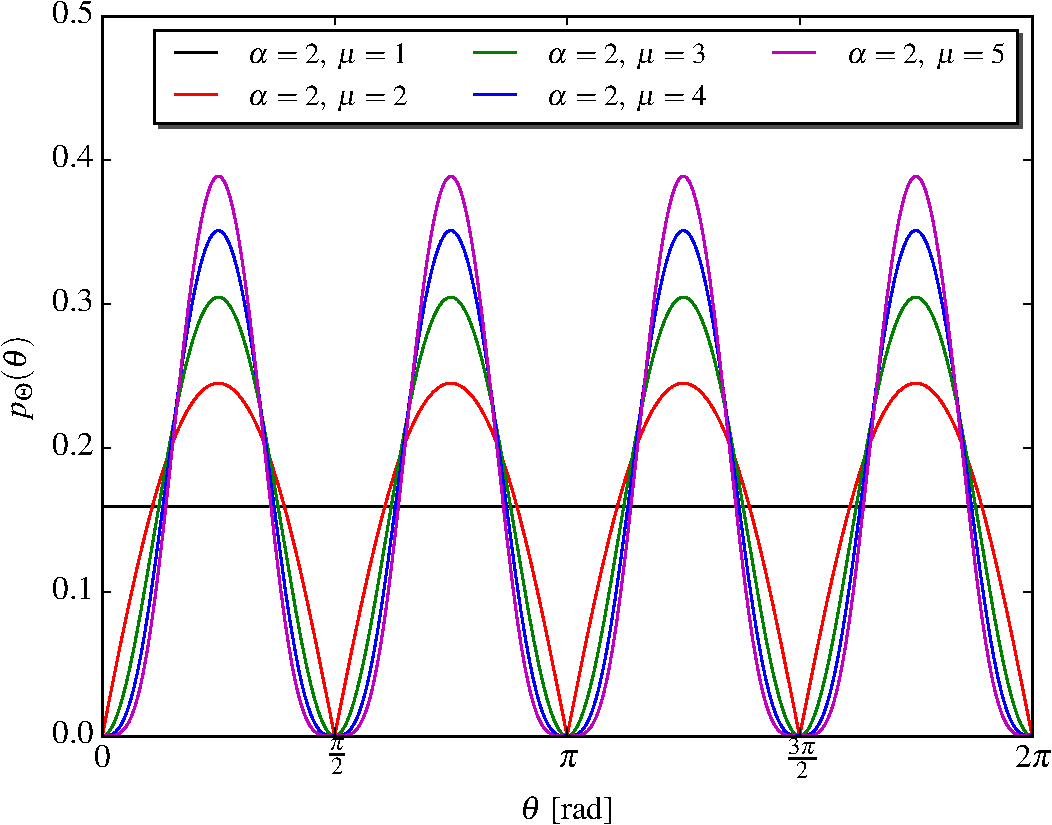
\includegraphics[scale=0.45]{images/phase_fig_1_linear.pdf}
        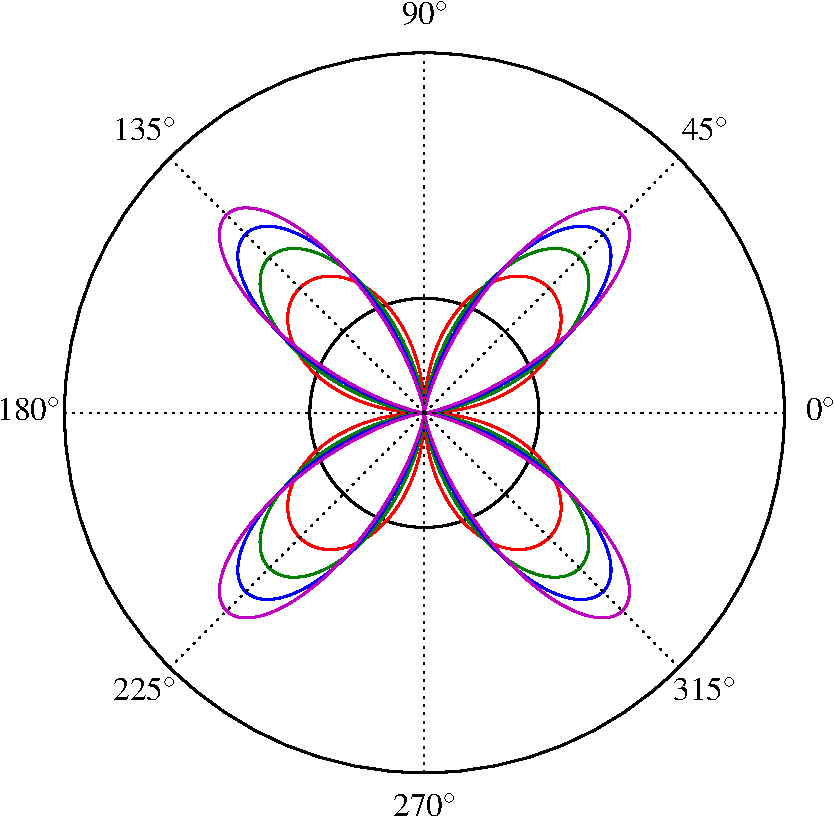
\includegraphics[scale=0.45]{images/phase_fig_1.pdf}
    \end{figure}
\end{frame}

\begin{frame}[plain]{Phase Density Function}
    \begin{center}
    \begin{figure}
        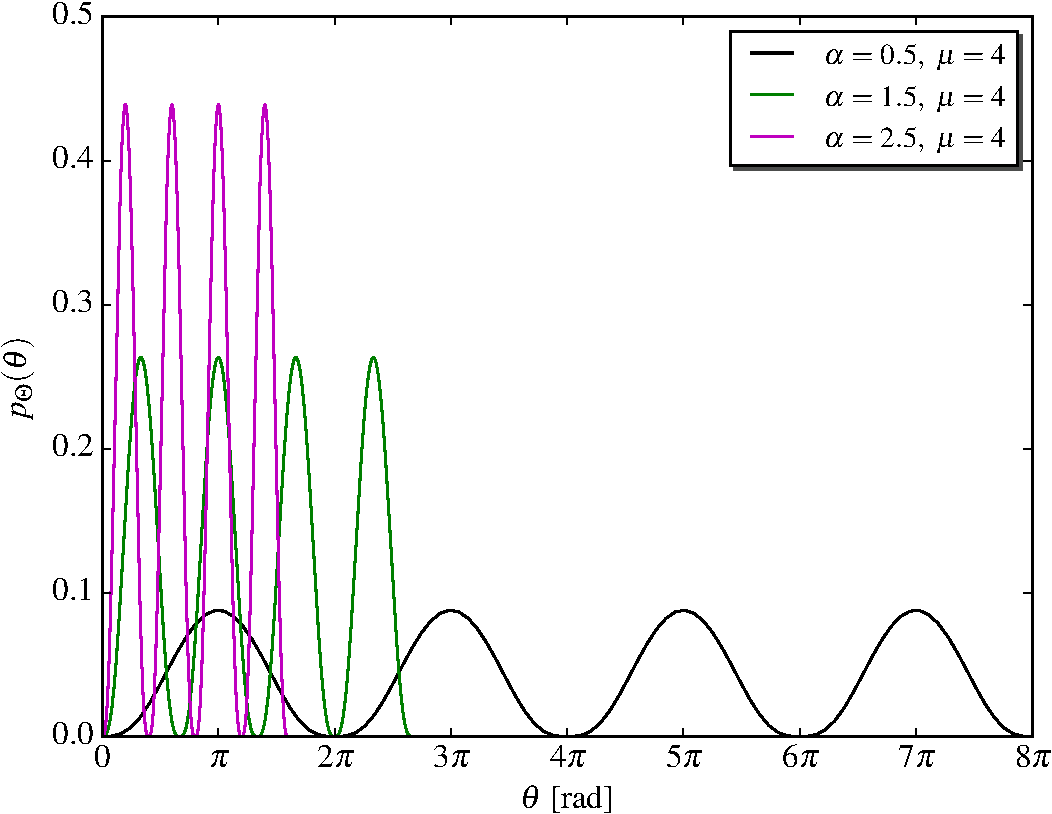
\includegraphics[scale=0.45]{images/phase_fig_2_linear.pdf}
        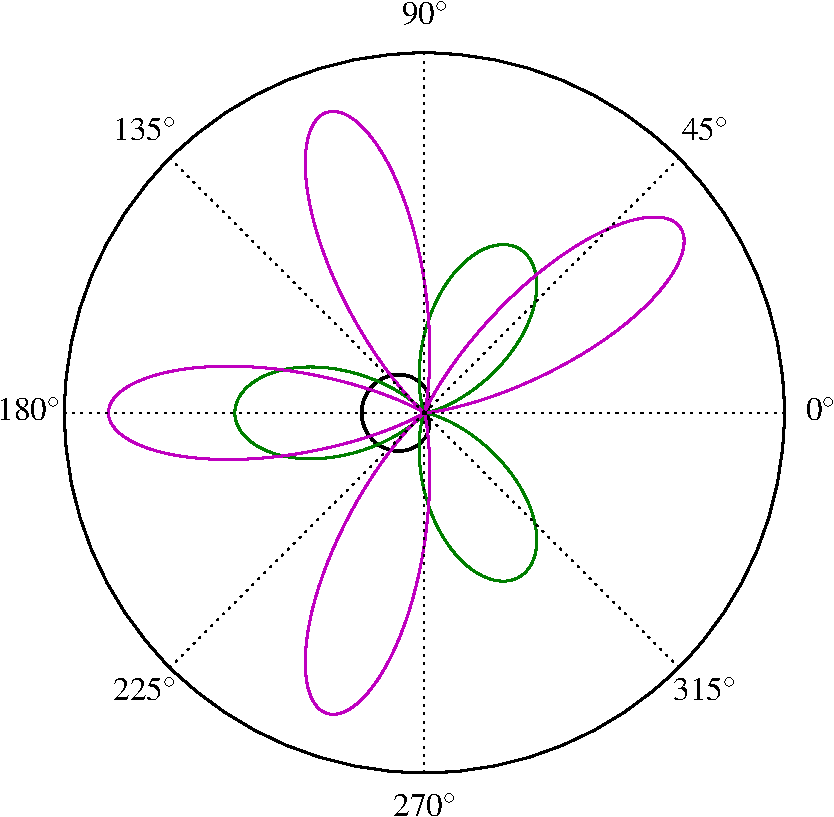
\includegraphics[scale=0.45]{images/phase_fig_2.pdf}
    \end{figure}
    \end{center}
\end{frame}


\section{Conclusions}
\begin{frame}{Conclusions and Future Works}
    \begin{itemize}
        \item A novel, approximate, and closed-form expression for the exponentiated Weibull joint envelope-phase distribution has been derived
        \item The exponentiated Weibull model fading finds applications in free-space optical communications channels subject to a variety of atmospheric turbulence conditions
        \item The proposed joint distribution may be applied to determine the performance, reliability, and high order statistics of such communications channels in many scenarios
        \item Further investigations may be conducted to derive an analytical expression for the marginal phase density function and to validate it with experimental data
    \end{itemize}
\end{frame}

\begin{frame}[plain]{Acknowledgments}
\begin{center}
\begin{figure}[H]
\begin{minipage}[h]{.3\linewidth}
%\hspace{-1.0cm}
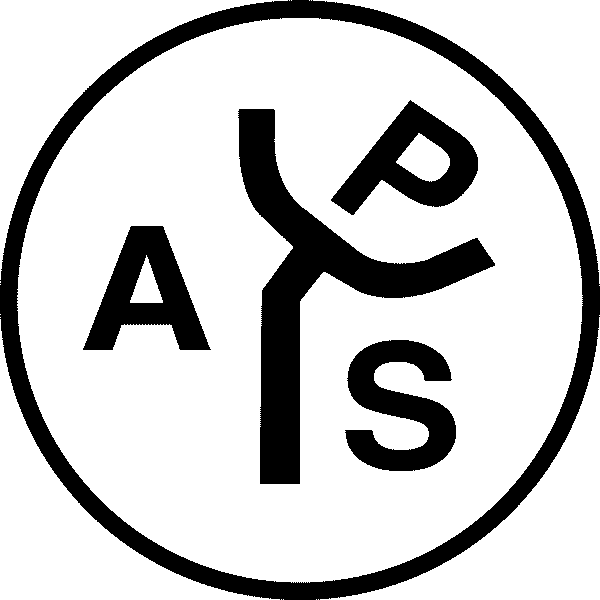
\includegraphics[scale=0.9]{images/aps.png}
\end{minipage}
\hspace{1.0cm}
%\begin{minipage}[h]{.01\linewidth}
%\end{minipage}
\begin{minipage}[h]{.4\linewidth}
%\hspace{-2.5cm}

\includegraphics[scale=2.5]{images/iecom.png}
\end{minipage}
\end{figure}
\end{center}

\hspace{3.5cm}

\begin{center}
\begin{figure}[H]
\begin{minipage}[h]{.3\linewidth}

\includegraphics[scale=0.6]{images/logoufcg.jpg}
\end{minipage}
\begin{minipage}[h]{.4\linewidth}
%\hspace{-2.5cm}

\includegraphics[scale=0.35]{images/psf.png} 
\end{minipage}
\end{figure}
\end{center}
    \texttt{Contact: jvmirca@gmail.com}
\end{frame}

\end{document}
